% !TeX TS-program = lualatex
\documentclass{article}
\usepackage{fontspec}
\usepackage[a4paper]{geometry}
\usepackage{babel} 



\usepackage{graphicx}
\graphicspath{ {./img/res/} }


\newcommand{\comment}[1]{}

\author{}
\title{}
\date{}


\begin{document}
	
	\maketitle
	
	\begin{center}
		Optimal-solved instances by time
		
		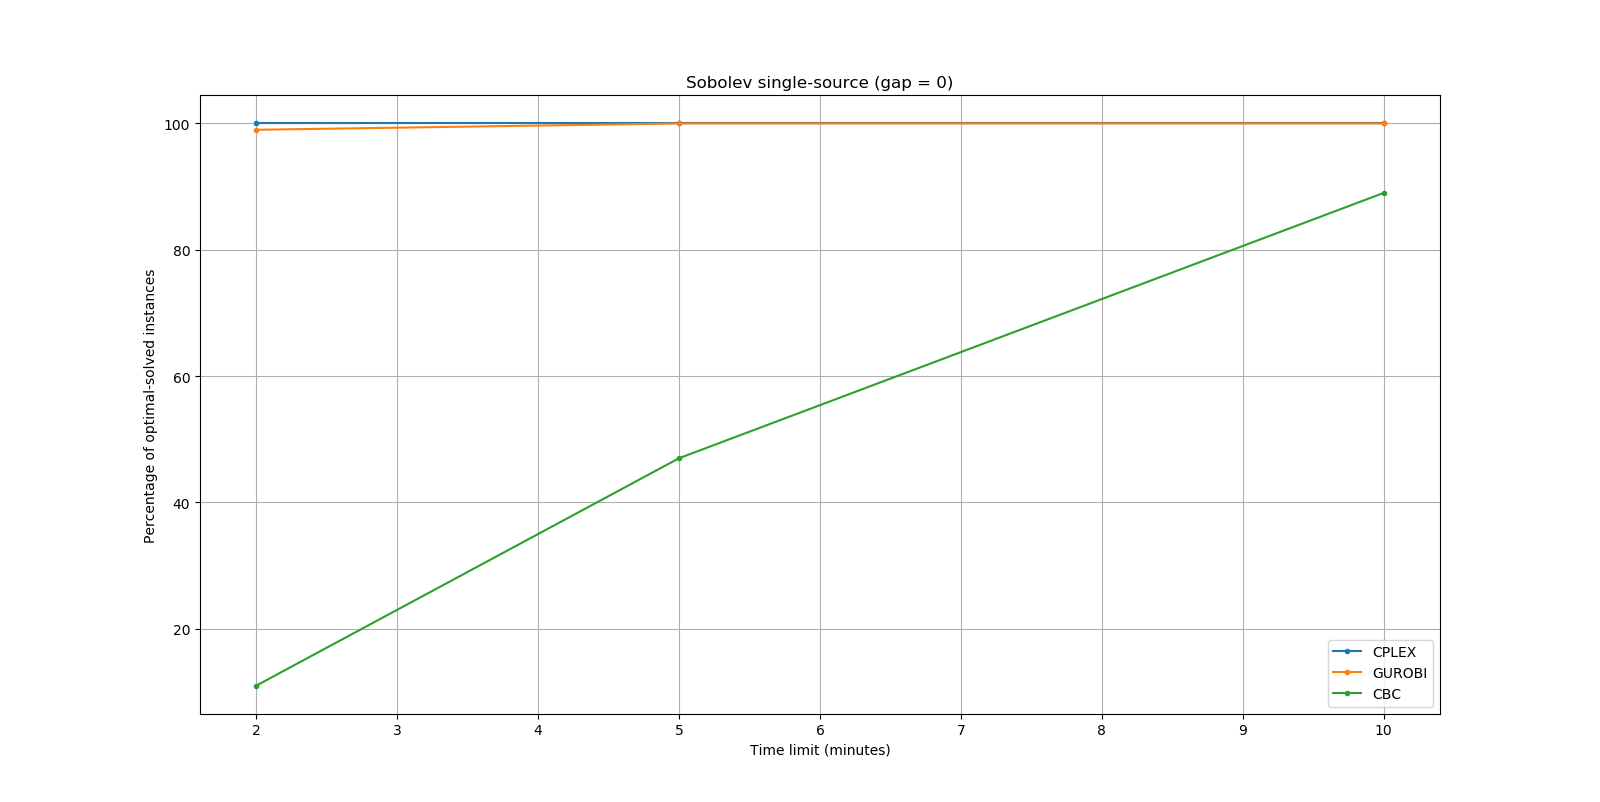
\includegraphics[width=\textwidth]{Sobolev SS - Optimal x Time}
		
		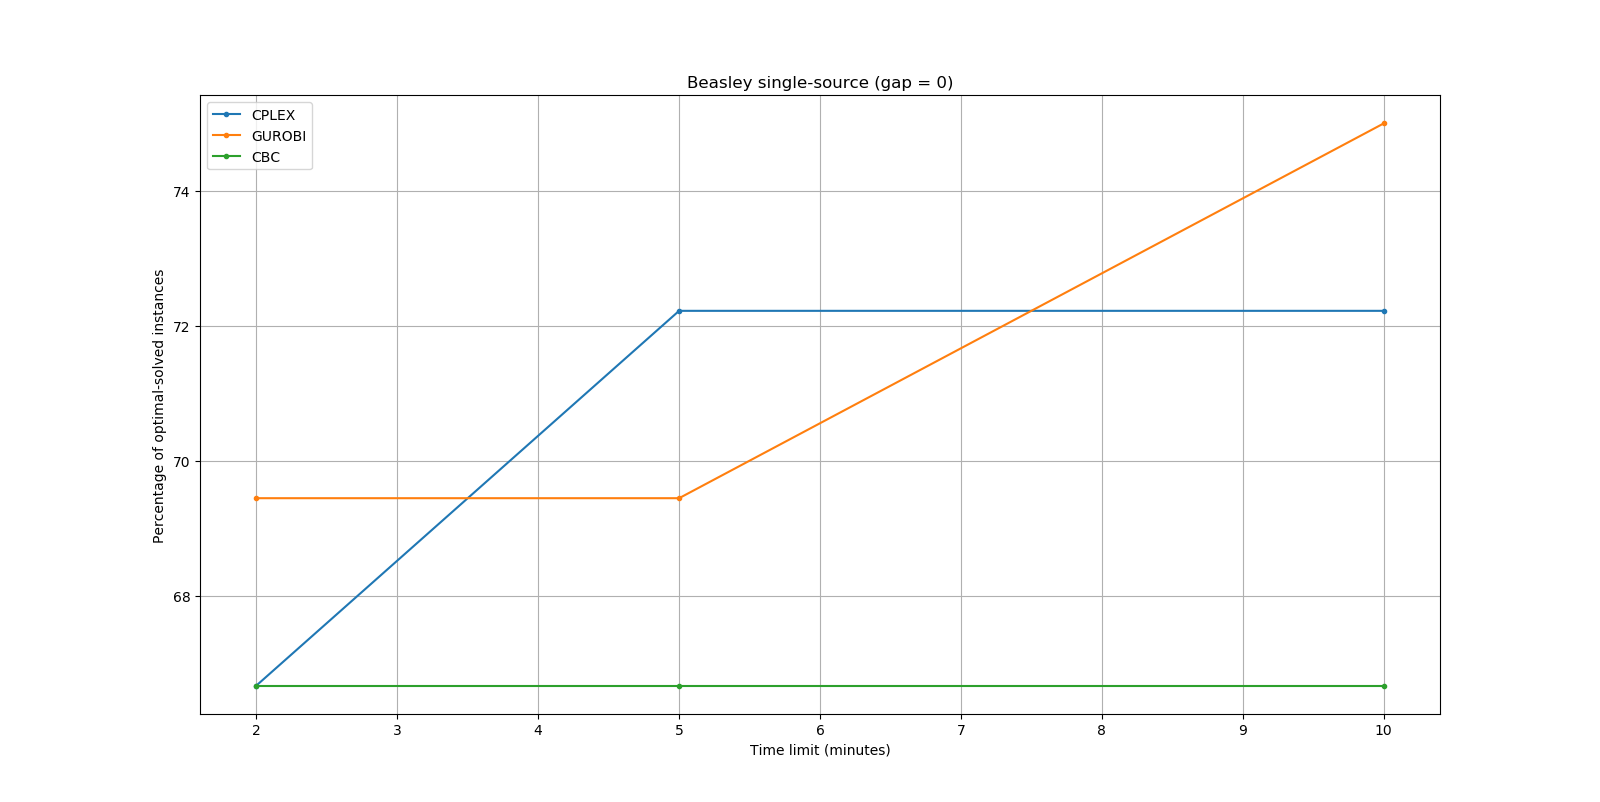
\includegraphics[width=\textwidth]{Beasley SS - Optimal x Time}
		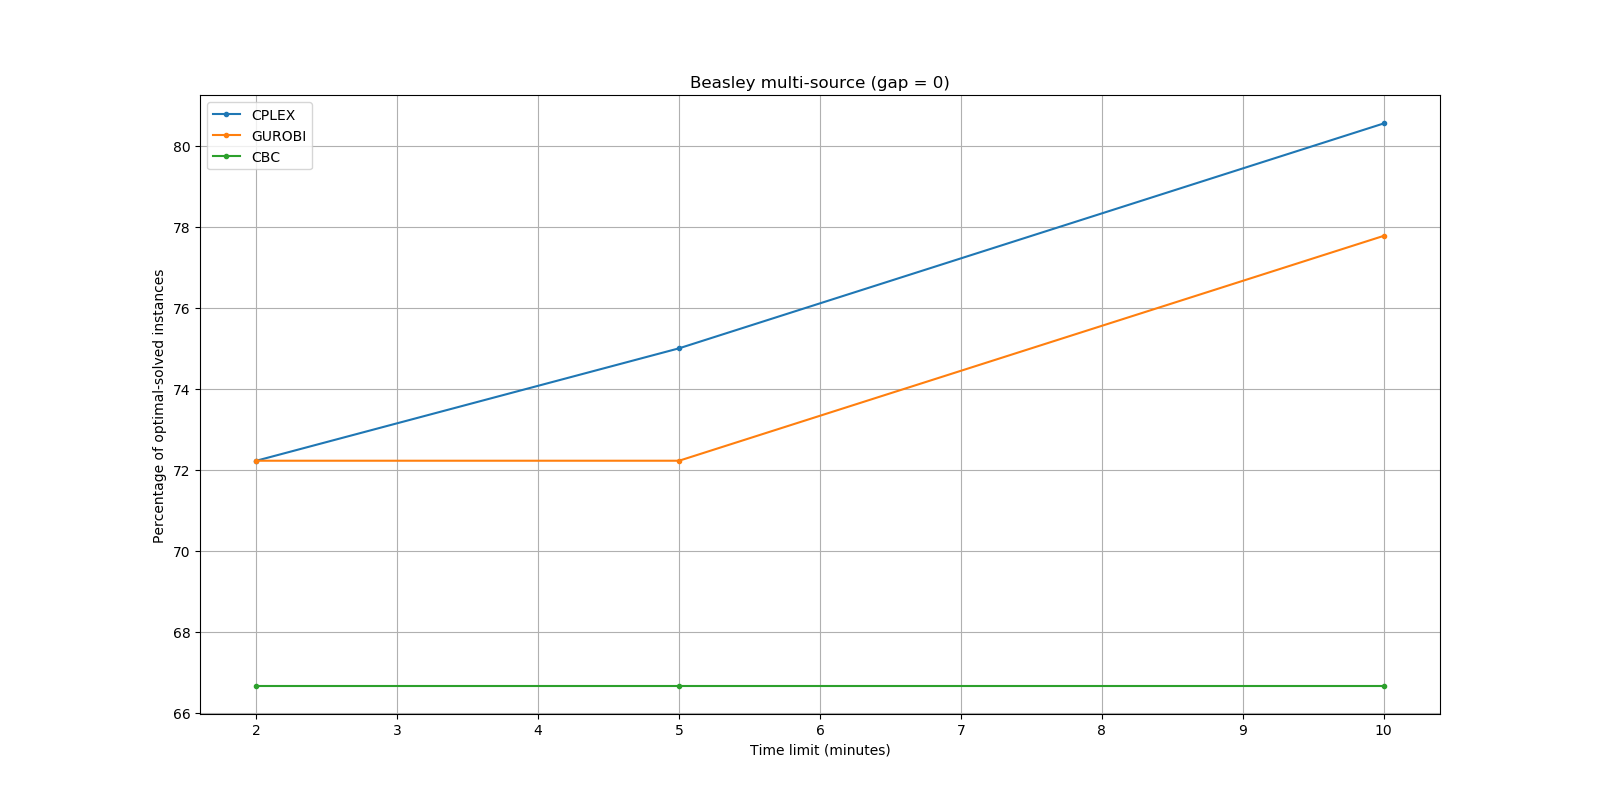
\includegraphics[width=\textwidth]{Beasley MS - Optimal x Time}
		
		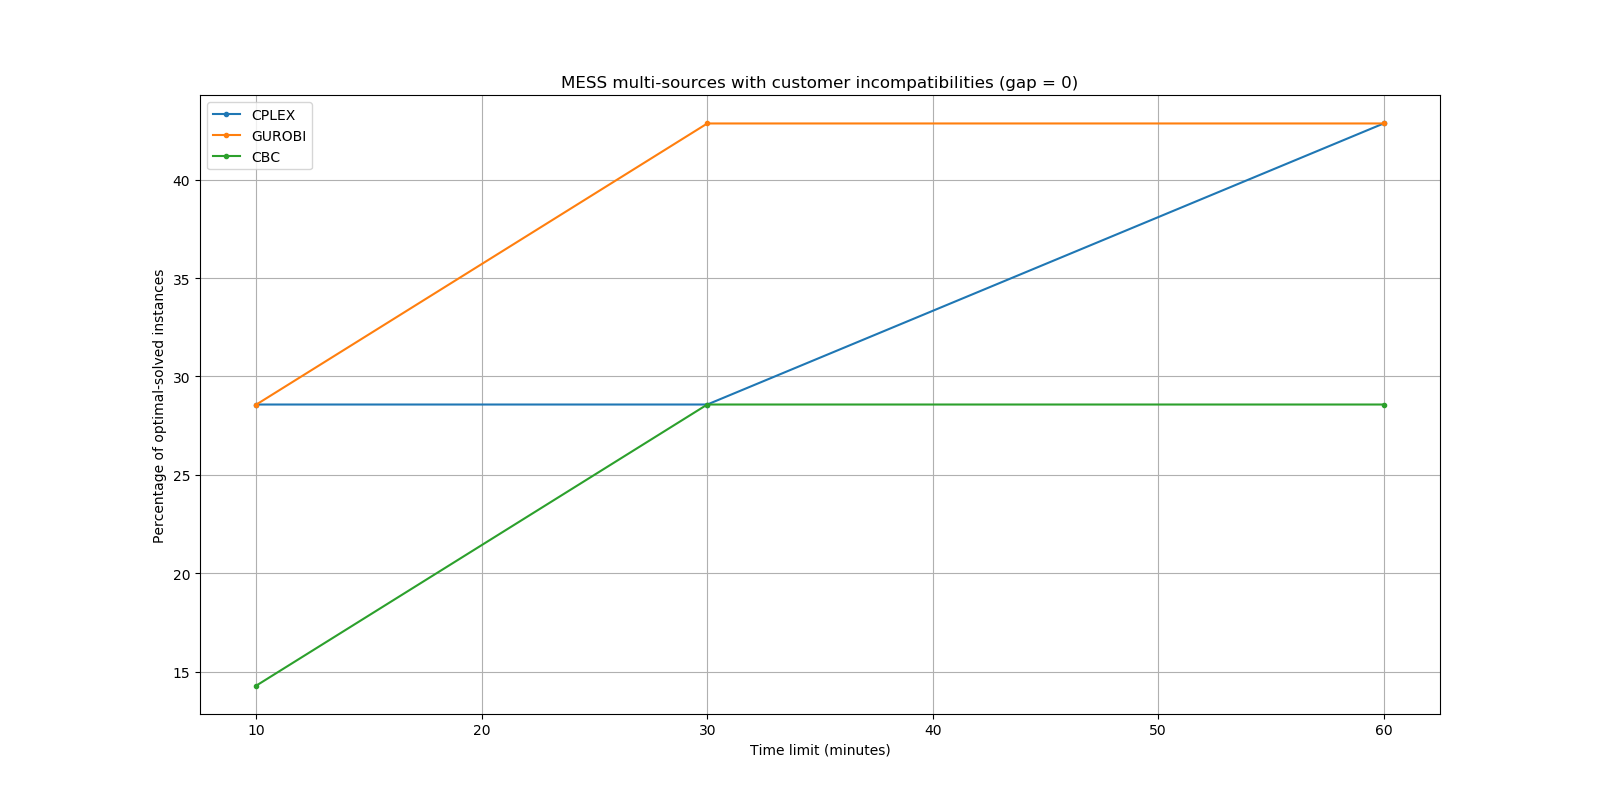
\includegraphics[width=\textwidth]{MESS MS CI - Optimal x Time}
		
	\end{center} 

	\newpage

	\begin{center}
		Beasley large instances average gap by time
		
		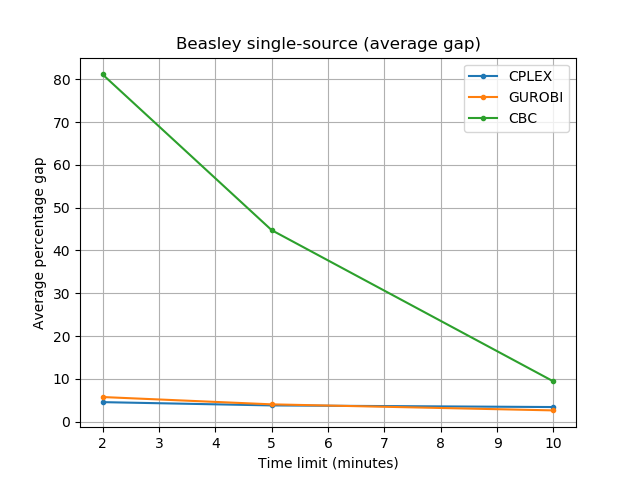
\includegraphics[width=0.49\textwidth]{Beasley SS large - Average gap x Time}
		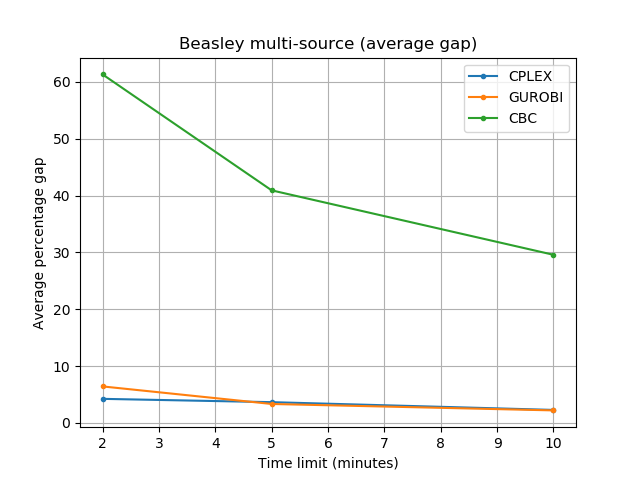
\includegraphics[width=0.49\textwidth]{Beasley MS large - Average gap x Time}
	\end{center}

	\begin{center}
		Beasley large instances average gap by nodes
		
		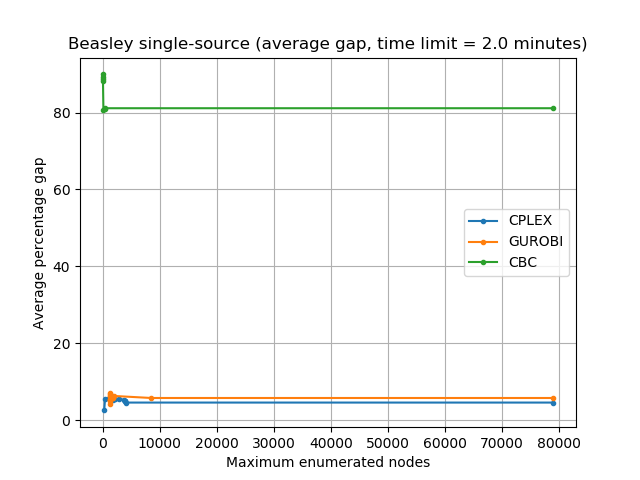
\includegraphics[width=0.32\textwidth]{Beasley SS large 120 - Average gap x Nodes}
		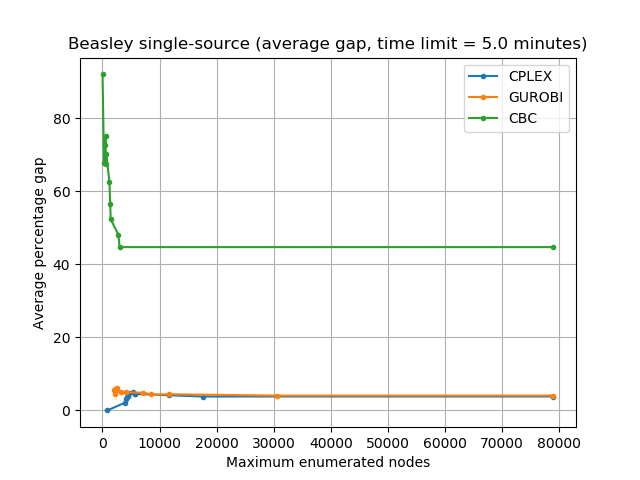
\includegraphics[width=0.32\textwidth]{Beasley SS large 300 - Average gap x Nodes}
		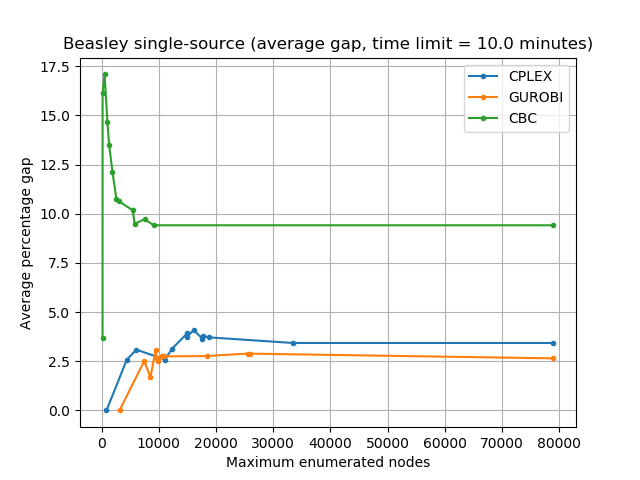
\includegraphics[width=0.32\textwidth]{Beasley SS large 600 - Average gap x Nodes}
		
		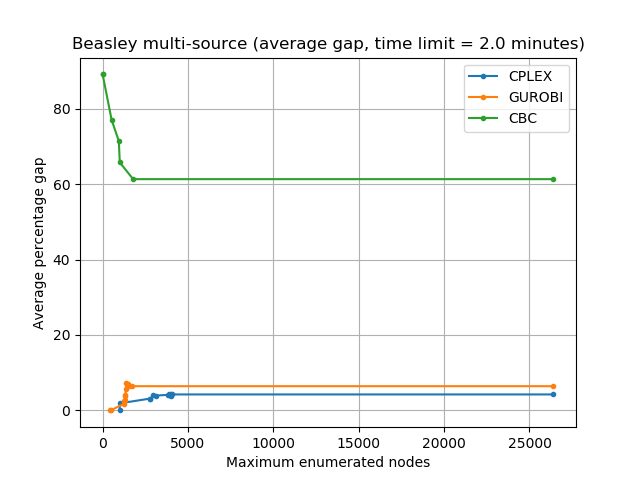
\includegraphics[width=0.32\textwidth]{Beasley MS large 120 - Average gap x Nodes}
		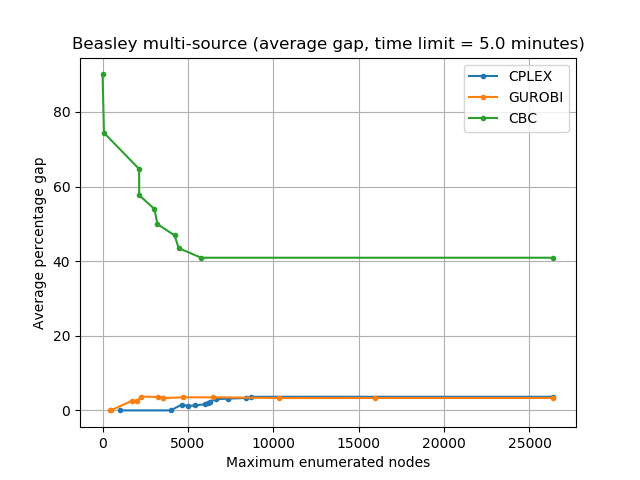
\includegraphics[width=0.32\textwidth]{Beasley MS large 300 - Average gap x Nodes}
		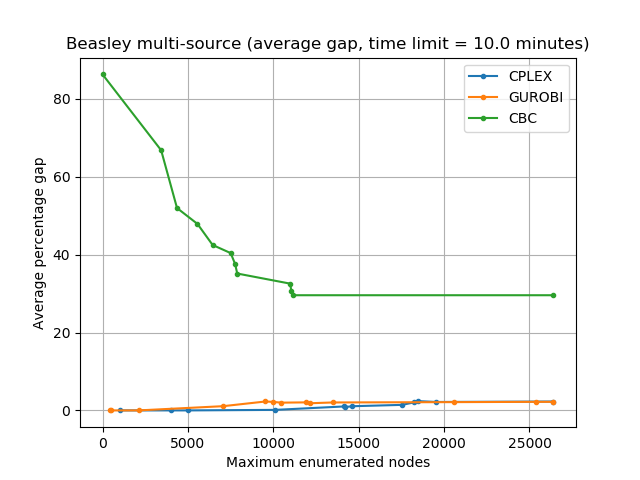
\includegraphics[width=0.32\textwidth]{Beasley MS large 600 - Average gap x Nodes}
	\end{center}

	\begin{center}
		Sobolev optimal-solved instances by nodes
		
		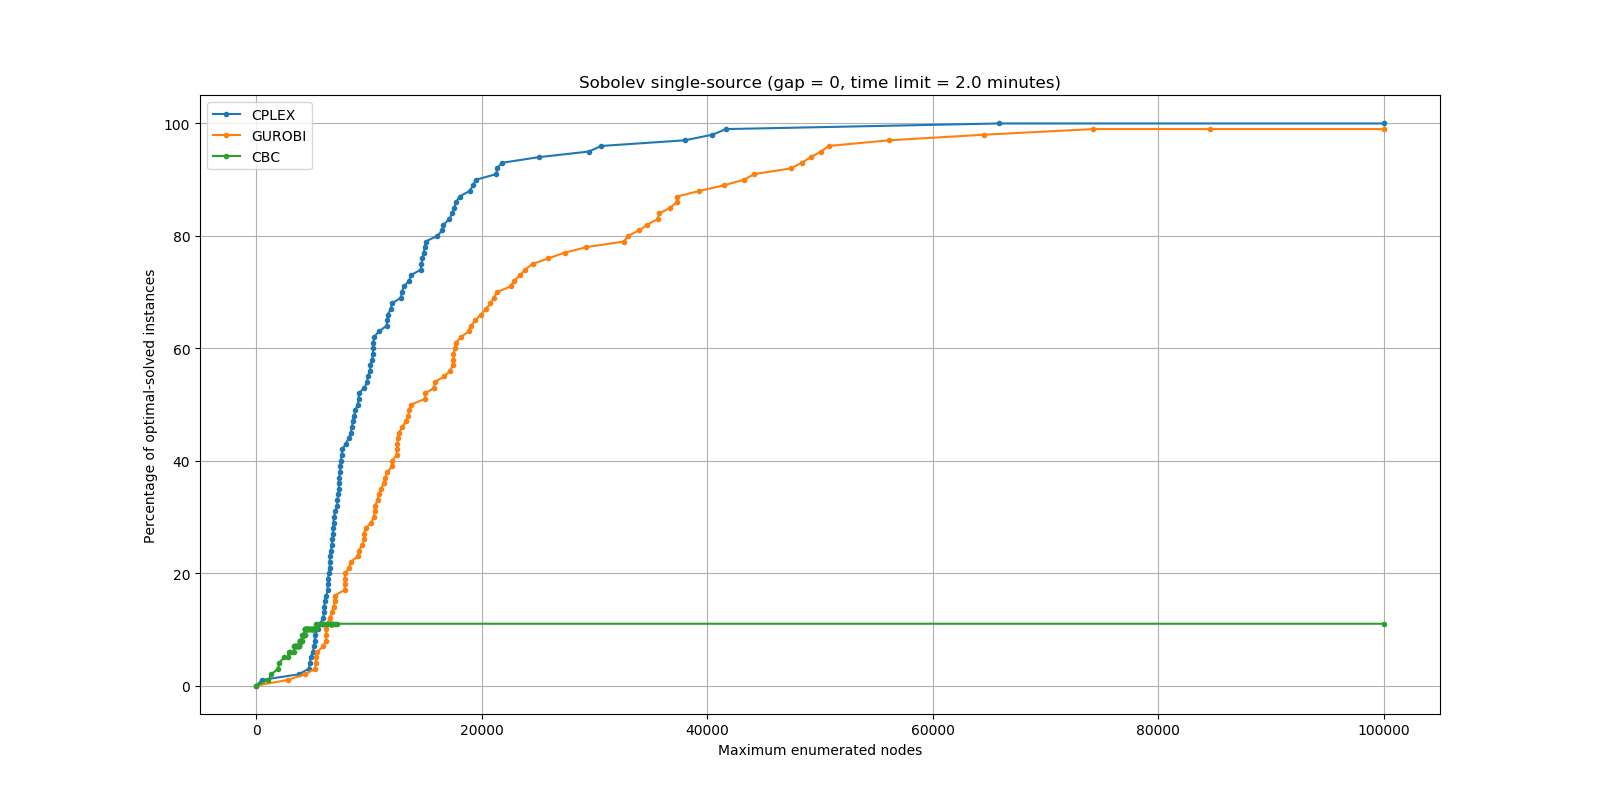
\includegraphics[width=0.32\textwidth]{Sobolev SS 120 - Optimal x Nodes}
		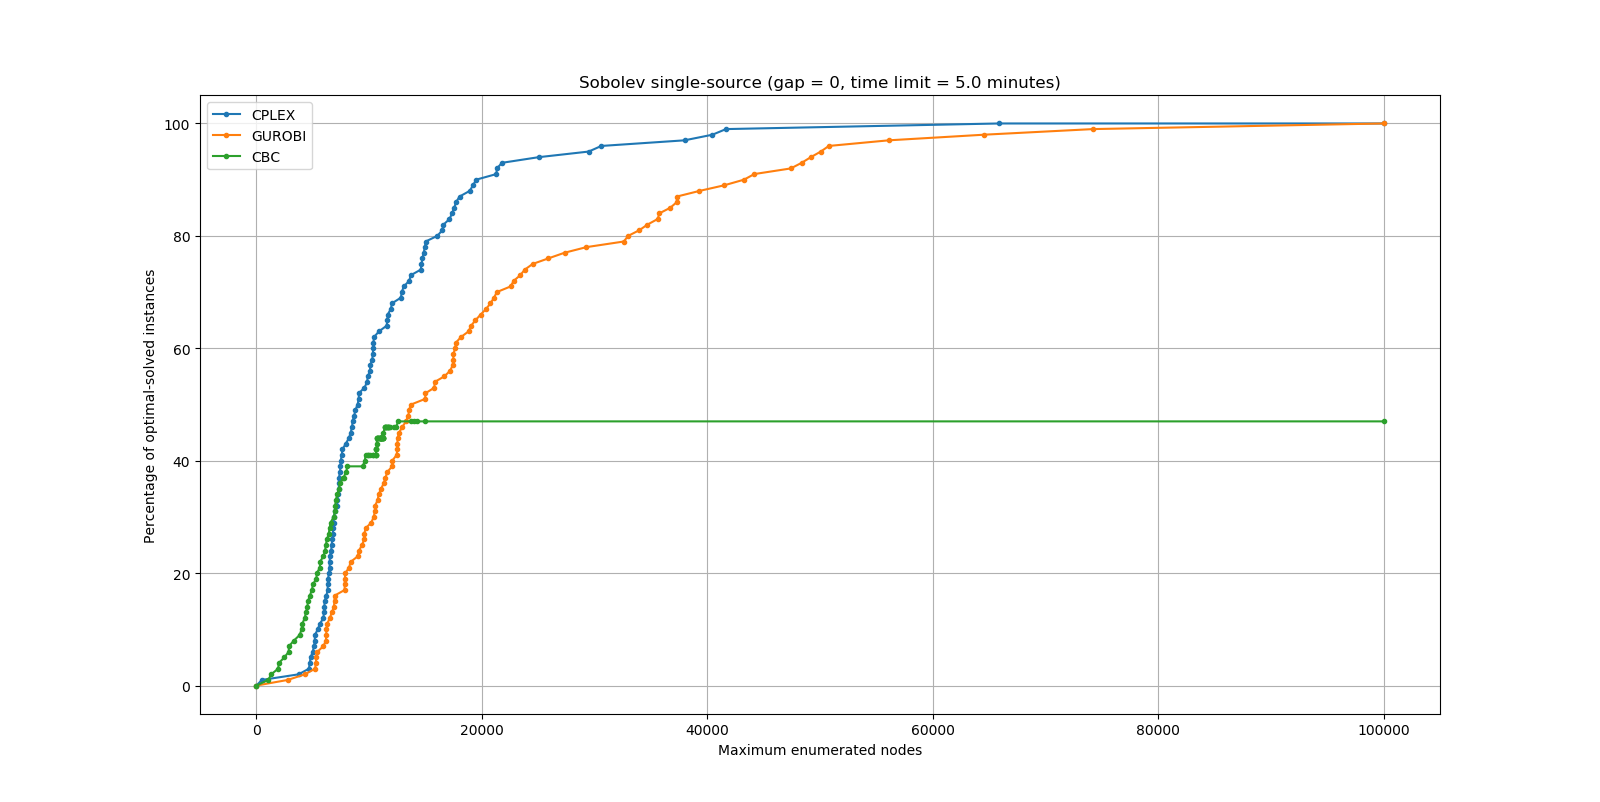
\includegraphics[width=0.32\textwidth]{Sobolev SS 300 - Optimal x Nodes}
		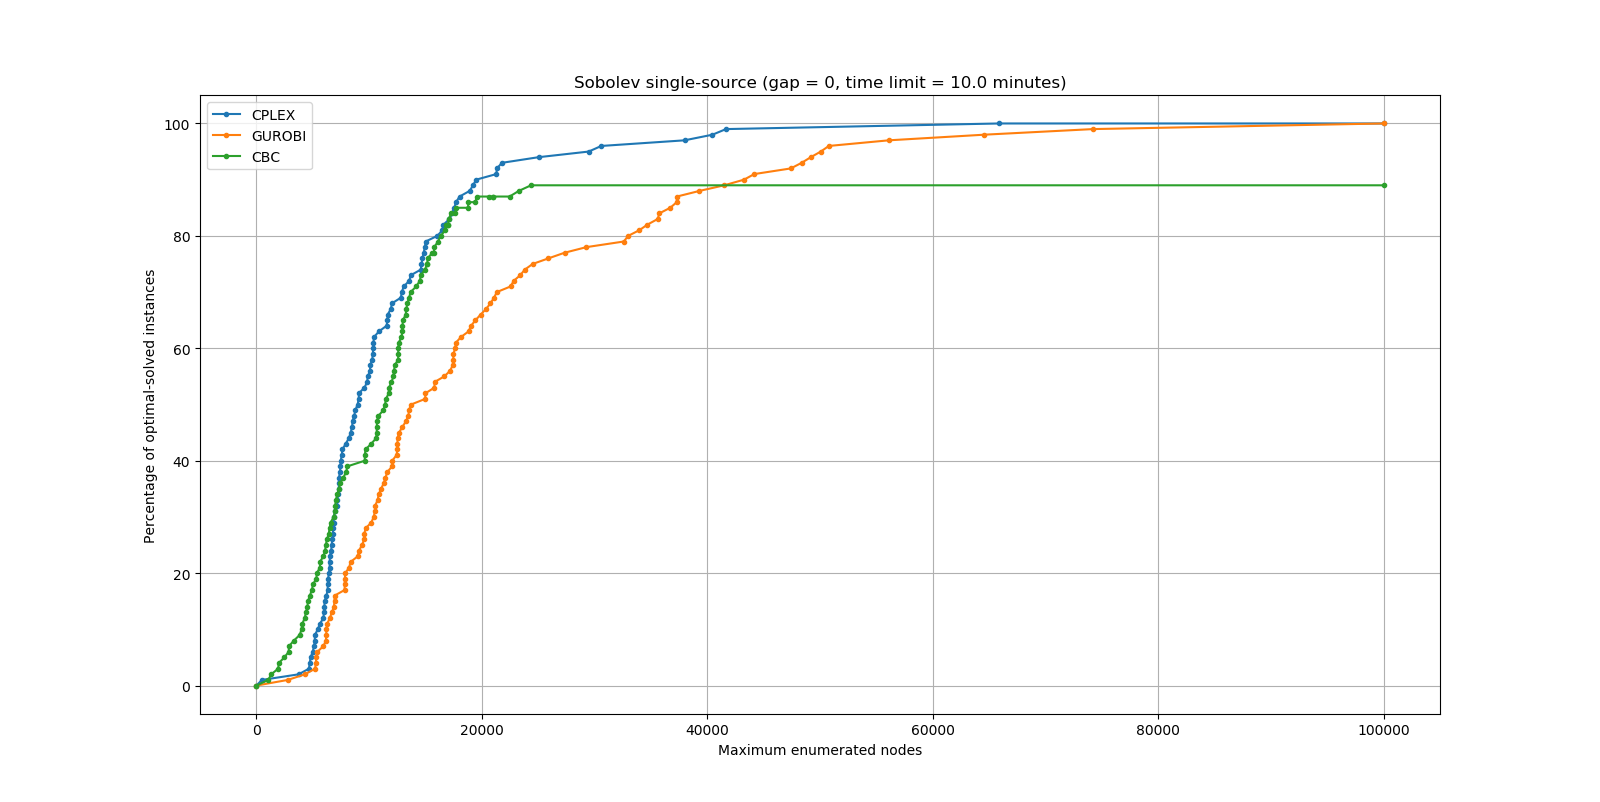
\includegraphics[width=0.32\textwidth]{Sobolev SS 600 - Optimal x Nodes}
		
	\end{center}

	CBC-solved Sobolev instances average percentual gap:
\\	120s time limit:	5.091517777160894
\\	300s time limit:	2.657761947500523
\\	600s time limit: 	0.0951064215085998	

	

\end{document}
